\documentclass[conference]{IEEEtran}
\IEEEoverridecommandlockouts
\usepackage{newtxtext,newtxmath}
\usepackage{cite}
\usepackage{amsmath}
\usepackage{algorithmic}
\usepackage{graphicx}
\usepackage{textcomp}
\usepackage{booktabs}
\usepackage{multirow}
\usepackage{pifont}
\usepackage{xcolor}
\renewcommand{\checkmark}{\ding{51}}
\def\BibTeX{{\rm B\kern-.05em{\sc i\kern-.025em b}\kern-.08em
    T\kern-.1667em\lower.7ex\hbox{E}\kern-.125emX}}
\begin{document}

\title{Semi-Supervised DeepSDF with Eikonal Regularization and Fourier Positional Encoding}

\author{\IEEEauthorblockN{Yu Taek Lee}
\IEEEauthorblockA{\textit{College of Computing and Data Science} \\
\textit{Nanyang Technological University}\\
Singapore \\
G2505374L \\
yutaek001@e.ntu.edu.sg}
}

\maketitle

\begin{abstract}
Neural implicit representations such as DeepSDF learn continuous signed distance functions for 3D shape reconstruction, but require dense signed distance supervision for every training point. We investigate whether Eikonal regularization can compensate for reduced supervision, and whether Fourier positional encoding (PE) helps or hurts in this regime. Using the corrected post-fix pipeline, we train on 299 ShapeNet shapes (airplane, chair, table) at supervision ratios from 5\% to 100\% and evaluate with Chamfer Distance (CD) and Normal Consistency (NC) on the training-set reconstructions. The main result is that Eikonal regularization improves label efficiency, but the strongest visually reliable operating point is 50\% supervision: EXP-03 reaches CD = 0.0288 and NC = 0.748, while preserving clearly recognizable structure. At 10\% supervision, the 3-seed no-PE run remains numerically competitive (CD = 0.0315 $\pm$ 0.0015, NC = 0.7288 $\pm$ 0.0032), but qualitative inspection shows that recognizable shape structure is less reliable than at 50\%. In contrast, Fourier PE is harmful at the 10\% supervision slice that we were able to retrain on the corrected pipeline: PE primarily collapses normal consistency (EXP-06 with $L=6$: NC = 0.5171 $\pm$ 0.0066; EXP-11 with $L=4$: NC = 0.6090) while leaving CD comparable to or only modestly worse than the no-PE 10\% baseline. Lowering the encoding frequency from $L=6$ to $L=4$ partially recovers NC at a clear CD cost. The originally-planned PE points at 5\% and 100\% supervision (and the second-order regularizer ablation) were not retrained under the post-fix QoS budget, so we restrict the PE conclusion to the 10\% supervision slice. We therefore conclude that Eikonal regularization is the useful ingredient for label reduction in this DeepSDF setup, whereas Fourier PE is not recommended at 10\% supervision.
\end{abstract}

\begin{IEEEkeywords}
DeepSDF, signed distance functions, Eikonal regularization, semi-supervised learning, positional encoding, 3D reconstruction
\end{IEEEkeywords}

%% ============================================================
\section{Introduction}
%% ============================================================

Learning 3D shape representations from data is a central problem in computer vision with applications in robotics, autonomous driving, and virtual reality. Traditional approaches such as voxel grids and point clouds suffer from resolution limitations and lack of surface continuity. Neural implicit representations address these issues by parameterizing shapes as continuous functions---typically signed distance functions (SDFs)---that can be queried at arbitrary resolution~\cite{deepsdf}.

DeepSDF~\cite{deepsdf} learns a neural network $f_\theta(z, x) \to s$ that maps a latent code $z$ and a 3D coordinate $x$ to a signed distance value $s$. Through an auto-decoder framework, per-shape latent codes are jointly optimized with the network weights, enabling the model to represent a distribution of shapes. However, DeepSDF requires dense signed distance supervision: every training point must have a ground-truth SDF value, which is expensive to obtain for real-world 3D data.

This supervision bottleneck motivates semi-supervised approaches that leverage geometric priors to reduce label requirements. The Eikonal equation $\|\nabla_x f(x)\| = 1$ is a fundamental property of signed distance functions~\cite{igr}. Enforcing this constraint on unsupervised points---those without SDF labels---provides a training signal derived purely from the geometry of the problem. If effective, this could substantially reduce the annotation effort for training neural implicit representations.

Separately, Fourier positional encoding (PE) has been shown to help multi-layer perceptrons (MLPs) learn high-frequency functions by mapping low-dimensional inputs to higher-dimensional sinusoidal features~\cite{nerf, fourierfeatures}. While this technique is standard in Neural Radiance Fields (NeRF), its interaction with SDF learning---particularly in semi-supervised settings---is less understood.

In this work, we systematically investigate two questions:
\begin{enumerate}
    \item Can Eikonal regularization reduce the need for signed distance supervision in DeepSDF, and by how much?
    \item Does Fourier positional encoding help or hurt reconstruction quality in this semi-supervised SDF setting?
\end{enumerate}

We report only the corrected post-fix experiments on 299 ShapeNet shapes (airplane, chair, table). Earlier runs produced under-informative supervision because the preprocessing pipeline sampled labels only inside a thin $\pm 0.1$ surface band; those runs are excluded from all tables and conclusions in this paper. After regenerating supervision with an 80/20 mix of near-surface multi-scale offsets and far-field signed-distance samples, the final experiment matrix becomes interpretable. Our key findings are:
\begin{itemize}
    \item \textbf{Eikonal regularization improves label efficiency}: relative to the non-Eikonal baseline (EXP-01, CD = 0.0361, NC = 0.729), Eikonal improves the full-label run (EXP-02, CD = 0.0295), gives the strongest overall no-PE result at 50\% supervision (EXP-03, CD = 0.0288, NC = 0.748), and keeps 10\% and 5\% supervision numerically competitive.
    \item \textbf{The 10\% no-PE regime is mixed rather than definitive}: EXP-04 (10\% supervision, 3 seeds) achieves CD = 0.0315 $\pm$ 0.0015 and NC = 0.7288 $\pm$ 0.0032, but qualitative inspection is noticeably less convincing than the 50\% run, so we do not treat 10\% supervision as the strongest visual operating point.
    \item \textbf{Fourier PE degrades NC at 10\% supervision}: post-fix EXP-06 ($L=6$, 3 seeds) achieves CD = 0.0308 $\pm$ 0.0012 and NC = 0.5171 $\pm$ 0.0066, and post-fix EXP-11 ($L=4$, single seed) achieves CD = 0.0432 and NC = 0.6090. CD remains close to the no-PE 10\% baseline; NC drops noticeably; lowering the PE frequency from $L=6$ to $L=4$ partially recovers NC at a clear CD cost. PE at 5\% and 100\% supervision was not retrained under the post-fix QoS budget, so the PE conclusion in this paper is restricted to 10\% supervision.
\end{itemize}

%% ============================================================
\section{Related Work}
%% ============================================================

\subsection{Neural Implicit Representations}

Neural implicit representations encode 3D geometry as the level set of a learned function. Occupancy Networks~\cite{occnet} predict binary inside/outside occupancy, while DeepSDF~\cite{deepsdf} regresses continuous signed distance values, enabling gradient-based surface extraction via marching cubes~\cite{marchingcubes}. DeepSDF's auto-decoder framework avoids the need for an encoder by directly optimizing per-shape latent codes during training. While effective, it requires dense SDF supervision at every training point.

\subsection{Geometric Regularization}

The Eikonal equation $\|\nabla_x f(x)\| = 1$ is a necessary condition for valid signed distance functions. Gropp et al.~\cite{igr} introduced Implicit Geometric Regularization (IGR), demonstrating that enforcing this constraint during training improves surface quality and enables learning from raw point clouds without SDF labels. This approach has been adopted in subsequent work on neural implicit surfaces~\cite{volsdf, neus}. In our work, we investigate whether Eikonal regularization can reduce the required number of supervised training points, assessing its effects across multiple supervision ratios.

SIREN~\cite{siren} takes a different approach to geometric regularization by using periodic activation functions (sinusoidal) instead of ReLU, which naturally satisfies certain differential equation constraints. However, SIREN requires architectural changes, whereas Eikonal regularization can be applied as a loss term to standard ReLU networks.

\subsection{Positional Encoding}

Fourier positional encoding was introduced in NeRF~\cite{nerf} to overcome the spectral bias of MLPs---their tendency to learn low-frequency functions first~\cite{spectralbias}. By mapping input coordinates through sinusoidal functions at multiple frequency bands, $\gamma(x) = [\sin(2^0\pi x), \cos(2^0\pi x), \ldots, \sin(2^{L-1}\pi x), \cos(2^{L-1}\pi x)]$, the network can represent high-frequency variations. Tancik et al.~\cite{fourierfeatures} provided a theoretical framework for this approach based on the Neural Tangent Kernel.

While Fourier features are standard in radiance field methods, their application to SDF learning is less established. NeRF operates in a supervised regime where every ray has a target color, and the network is evaluated primarily at points along training rays. In contrast, SDF evaluation via marching cubes requires querying the network on a dense grid that includes regions far from the training data distribution, creating an extrapolation challenge for high-frequency encodings.

%% ============================================================
\section{Method}
\label{sec:method}
%% ============================================================

\subsection{Problem Formulation}

Given a dataset of 3D shapes, we aim to learn a function $f_\theta: \mathbb{R}^{d_z} \times \mathbb{R}^3 \to \mathbb{R}$ that maps a shape-specific latent code $z_i \in \mathbb{R}^{d_z}$ and a spatial coordinate $x \in \mathbb{R}^3$ to the signed distance to the shape's surface. For each shape $i$, we have:
\begin{itemize}
    \item \textbf{Supervised points}: $\{(x_j, s_j)\}_{j=1}^{N_s}$ with ground-truth SDF values (see Section~\ref{sec:dataset} for the exact sampling procedure)
    \item \textbf{Unsupervised points}: $\{x_k\}_{k=1}^{N_u}$ with coordinates only
\end{itemize}
During preprocessing, each shape is sampled to produce a fixed pool of 250{,}000 supervised points and a separate pool of 250{,}000 unsupervised points. The supervision ratio $r$ controls the fraction of the supervised pool that is retained: at $r = 0.1$ only 25{,}000 supervised points are used, while all 250{,}000 unsupervised points remain available. At $r = 1.0$ the full supervised pool is used alongside the full unsupervised pool. Each training batch samples half its points from the supervised set and half from the unsupervised set. We investigate $r \in \{0.05, 0.10, 0.50, 1.0\}$.

\subsection{Architecture}

We use an 8-layer MLP with hidden dimension 512, following the DeepSDF architecture~\cite{deepsdf}. A skip connection concatenates the input to the activations at layer 4. Each shape is associated with a learnable latent code $z_i \in \mathbb{R}^{256}$, initialized from $\mathcal{N}(0, 0.01^2)$ and jointly optimized with the network weights (auto-decoder). The final layer produces a scalar SDF value without activation, with weights initialized from $\mathcal{N}(0, 1/\sqrt{512})$ and bias set to 0.1 to approximate a sphere.

When Fourier PE is enabled, input coordinates are transformed as:
\begin{equation}
    \gamma(x) =
    [\sin(2^0 \pi x), \cos(2^0 \pi x), \ldots,
    \sin(2^{L-1} \pi x), \cos(2^{L-1} \pi x)]
\end{equation}
where $L$ is the number of frequency levels. This maps each 3D coordinate from $\mathbb{R}^3$ to $\mathbb{R}^{6L}$. The network input becomes $[z_i; \gamma(x)]$ instead of $[z_i; x]$. We test $L=4$ (24-dimensional) and $L=6$ (36-dimensional).

\subsection{Loss Functions}

The total training loss combines four terms:
\begin{equation}
    \mathcal{L} = \mathcal{L}_{\text{sdf}} + \lambda_{\text{eik}}(t) \cdot \mathcal{L}_{\text{eik}} + \lambda_z \cdot \mathcal{L}_z + \lambda_{\text{2nd}} \cdot \mathcal{L}_{\text{2nd}}
\end{equation}

\textbf{SDF loss} ($\mathcal{L}_{\text{sdf}}$): L1 regression on supervised points only:
\begin{equation}
    \mathcal{L}_{\text{sdf}} = \frac{1}{N_s} \sum_{j=1}^{N_s} |f_\theta(z_i, x_j) - s_j|
\end{equation}

\textbf{Eikonal loss} ($\mathcal{L}_{\text{eik}}$): Enforces $\|\nabla_x f\| = 1$ on all points (supervised and unsupervised), providing geometric regularization from unlabeled data:
\begin{equation}
    \mathcal{L}_{\text{eik}} = \frac{1}{N_s + N_u} \sum_{k} \left(\|\nabla_x f_\theta(z_i, x_k)\| - 1\right)^2
\end{equation}

\textbf{Latent regularization} ($\mathcal{L}_z$): Prevents latent code drift:
\begin{equation}
    \mathcal{L}_z = \|z_i\|^2
\end{equation}

\textbf{Second-order loss} ($\mathcal{L}_{\text{2nd}}$): Optionally penalizes the divergence of the gradient field to encourage smoother surfaces:
\begin{equation}
    \mathcal{L}_{\text{2nd}} = \frac{1}{N} \sum_k |\nabla \cdot \nabla_x f_\theta(z_i, x_k)|
\end{equation}

\subsection{Eikonal Warmup Schedule}

The Eikonal weight uses a linear warmup to prevent the gradient norm constraint from dominating before the network learns basic geometry from $\mathcal{L}_{\text{sdf}}$:
\begin{equation}
    \lambda_{\text{eik}}(t) = \lambda_{\text{eik}} \cdot \min\left(1, \frac{t}{T_w}\right)
\end{equation}
where $T_w$ is ratio-dependent: 100 epochs for $r \geq 0.5$, 150 epochs for $r = 0.1$, and 200 epochs for $r = 0.05$. Lower supervision ratios require longer warmup because fewer supervised points provide weaker initial geometry signal.

\subsection{Training Procedure}

Training iterates over all shapes per epoch, sampling a batch of 16{,}384 points per shape split evenly between supervised and unsupervised samples. We use the Adam optimizer with learning rate $5 \times 10^{-4}$, decayed by $0.5\times$ every 500 epochs, and gradient clipping at $\max\_norm = 1.0$.

Default hyperparameters are $\lambda_{\text{eik}} = 0.1$, $\lambda_z = 10^{-4}$, and $\lambda_{\text{2nd}} = 0$ (disabled). EXP-01 and EXP-02 train for 3{,}000 epochs; the post-fix priority retrains (EXP-03/04/05/06/11, including the EXP-04 and EXP-06 multi-seed replicates) train for 1{,}500 epochs to fit the QoS budget.

%% ============================================================
\section{Experiments}
%% ============================================================

\subsection{Dataset}
\label{sec:dataset}

We use 300 shapes from ShapeNet~\cite{shapenet} spanning three categories (100 airplanes, 100 chairs, 100 tables). Preprocessing normalizes each mesh to the unit sphere and then samples two point pools per shape:
\begin{itemize}
    \item \textbf{Supervised pool} (250{,}000 points). An 80/20 mix:
    \begin{itemize}
        \item \emph{Near-surface (200K)} points generated by multi-scale normal offsets at scales $\epsilon \in \{0.005, 0.01, 0.05\}$ with multipliers $\{-2,-1,1,2\}$, yielding SDF magnitudes up to $|s|=0.1$.
        \item \emph{Far-field (50K)} points sampled uniformly inside the unit sphere with exact signed distance from \texttt{trimesh.proximity.signed\_distance}. Trimesh's convention is positive-inside/negative-outside; we invert the sign to match the project convention (positive-outside/negative-inside).
    \end{itemize}
    Meshes with more than 15{,}000 faces are decimated to 10{,}000 faces before the far-field query to keep preprocessing tractable.
    \item \textbf{Unsupervised pool} (250{,}000 points). Uniform in the unit sphere, coordinates only; used by the Eikonal term.
\end{itemize}
Each mesh is processed with a deterministic per-mesh seed derived from the global seed and the mesh name, so parallel preprocessing is reproducible. One airplane mesh (airplane\_0077) had degenerate triangles that caused \texttt{signed\_distance} to stall beyond 30 minutes; it was dropped from the pipeline, leaving 299 shapes. All 299 shapes are used for training (\texttt{train\_split}~=~1.0); we do not hold out a separate test set in the post-fix pipeline, because the experiment target is a stress test of label efficiency and PE interactions on the training objective rather than generalization to unseen shapes. Reported CD/NC are therefore reconstruction metrics over the training set, and should be interpreted accordingly.

For reduced-supervision runs, supervised points are subsampled to the target ratio (e.g.\ 10\% retains 25{,}000 labeled points) while all 250{,}000 unsupervised points remain available for Eikonal regularization.

\subsection{Evaluation Metrics}

For each trained model we extract a mesh per shape via marching cubes~\cite{marchingcubes} on the SDF field clipped to the unit sphere. All post-fix evaluations are run at resolution $128^3$. We report two metrics over the 299 training shapes:

\textbf{Chamfer Distance (CD)}: L1 bidirectional mean nearest-neighbor distance between 30{,}000 points sampled from predicted and ground-truth meshes. Lower is better.

\textbf{Normal Consistency (NC)}: Mean absolute dot product between normals at matched nearest-neighbor pairs. Higher is better (maximum 1.0).

Volumetric IoU and Eikonal Deviation were part of the original plan but were not computed; we discuss this explicitly in Section~\ref{sec:limitations}.

\subsection{Experiment Design}

Table~\ref{tab:experiments} summarizes the final corrected post-fix experiment matrix used in this report. We vary supervision ratio ($r \in \{5\%, 10\%, 50\%, 100\%\}$), Eikonal regularization, and Fourier PE frequency ($L \in \{4, 6\}$). Key comparisons are EXP-03 vs.\ EXP-01/02 (label reduction without PE), EXP-04 vs.\ EXP-03 (what is lost when supervision drops from 50\% to 10\%), EXP-06 vs.\ EXP-04 (PE effect at 10\% supervision), and EXP-11 vs.\ EXP-06 (PE frequency follow-up at 10\% supervision). Two configurations were multi-seeded (seeds 42, 123, 456): EXP-04 and EXP-06. Their coefficients of variation remain below the project threshold of 0.2, so no seed expansion was required. The originally-planned PE points at 100\% and 5\% supervision (EXP-09/EXP-07/EXP-10/EXP-12) and the second-order regularizer ablation (EXP-08) were not retrained under the post-fix compute budget; pre-fix exploratory results for those slots are not reported as final numbers.

\begin{table}[t]
\centering
\caption{Final corrected post-fix experiment set actually used in this paper. All experiments use Eikonal regularization except EXP-01. Originally-planned slots EXP-07/08/09/10/12 were not retrained under the post-fix QoS budget and are excluded from all tables, figures, and conclusions.}
\label{tab:experiments}
\renewcommand{\arraystretch}{1.1}
\scriptsize
\resizebox{\columnwidth}{!}{%
\begin{tabular}{@{}lccccl@{}}
\toprule
ID & $r$ & Eik & PE & Seeds & Purpose \\
\midrule
01 & 100\% & -- & -- & 42 & Baseline \\
02 & 100\% & \checkmark & -- & 42 & Full-label Eikonal \\
03 & 50\% & \checkmark & -- & 42 & Half labels \\
04 & 10\% & \checkmark & -- & 42,123,456 & Low-label no-PE \\
05 & 5\% & \checkmark & -- & 42 & Minimal labels no-PE \\
06 & 10\% & \checkmark & $L$=6 & 42,123,456 & Low-label PE \\
11 & 10\% & \checkmark & $L$=4 & 42 & Lower PE freq, low labels \\
\bottomrule
\end{tabular}
\!}
\end{table}

All experiments were trained on a single NVIDIA A40 GPU in the NTU TC2 cluster. EXP-01 and EXP-02 used 3{,}000 epochs; the post-fix priority retrains (EXP-03/04/05/06/11) used 1{,}500 epochs to fit the TC2 QoS budget. Hyperparameters are otherwise shared across runs: $\lambda_{\text{eik}}=0.1$, $\lambda_z = 10^{-4}$, batch size 16{,}384, Adam with learning rate $5 \times 10^{-4}$, gradient clipping at $\max\_\text{norm}=1.0$, and the ratio-dependent Eikonal warmup from Section~\ref{sec:method}.

%% ============================================================
\section{Results}
%% ============================================================

All numbers in this section are from the corrected post-fix pipeline: all
reported runs were retrained on regenerated data with 80\% near-surface
multi-scale offsets plus 20\% far-field signed-distance samples, and were
evaluated on 299 training shapes. Earlier wrong-pipeline runs are excluded
from every table and conclusion in this paper.

\subsection{Eikonal Improves Label Efficiency, but 50\% Is the Clearest Visual Point}
\label{sec:eikonal_results}

Table~\ref{tab:results} summarizes the final corrected experiment set. The
non-PE progression is favorable overall: the vanilla baseline (EXP-01) reaches
CD = 0.0361 and NC = 0.729, while adding Eikonal at full supervision (EXP-02)
improves CD to 0.0295. The strongest no-PE operating point is EXP-03 at 50\%
supervision, which attains the best CD/NC pair among the non-PE runs
(0.0288 / 0.748). This is also the configuration whose reconstructions remain
the most convincingly recognizable in the qualitative figures.

\begin{table}[t]
\centering
\caption{Final corrected post-fix results. Values are reported exactly as used
in the final report narrative: single-seed rows are per-shape means over 299
training shapes; multi-seed rows are means of per-seed means.}
\label{tab:results}
\renewcommand{\arraystretch}{1.1}
\footnotesize
\begin{tabular}{@{}llcc@{}}
\toprule
ID & Config & CD ($\downarrow$) & NC ($\uparrow$) \\
\midrule
\multicolumn{4}{@{}l}{\textit{Without Positional Encoding}} \\
01 & 100\%, no Eik & 0.0361 & 0.729 \\
02 & 100\% + Eik & 0.0295 & 0.721 \\
03 & 50\% + Eik & 0.0288 & 0.748 \\
04 & 10\% + Eik (3-seed) & 0.0315{\scriptsize$\pm$0.0015} & 0.729{\scriptsize$\pm$0.003} \\
05 & 5\% + Eik & 0.0344 & 0.724 \\
\midrule
\multicolumn{4}{@{}l}{\textit{With Fourier Positional Encoding (10\% supervision only post-fix)}} \\
06 & 10\% + Eik + PE $L=6$ (3-seed) & 0.0308{\scriptsize$\pm$0.0012} & 0.5171{\scriptsize$\pm$0.0066} \\
11 & 10\% + Eik + PE $L=4$ & 0.0432 & 0.6090 \\
\bottomrule
\end{tabular}
\end{table}

The no-PE label-efficiency trend is therefore positive but not monotone in the
way one might have expected before examining the meshes. At 10\% supervision,
EXP-04 remains numerically competitive with EXP-01 and shows healthy seed
stability, but the per-shape comparisons reveal that it often preserves only
coarse category identity. By contrast, EXP-03 at 50\% supervision much more
reliably preserves the original object structure. For the final written claim,
we therefore treat 50\% + Eikonal as the clearest supported label-efficiency
result, and 10\% + Eikonal as promising but visually weaker.

Qualitative inspection (Figs.~\ref{fig:qualitative} and
\ref{fig:mesh_comparison}) changes the emphasis of the story. The 50\% Eikonal
run preserves the original structure clearly across categories, whereas the 10\%
run often retains only a coarse silhouette. This is exactly why the final
conclusion is more conservative than a metric-only reading of EXP-04.

\begin{figure}[t]
    \centering
    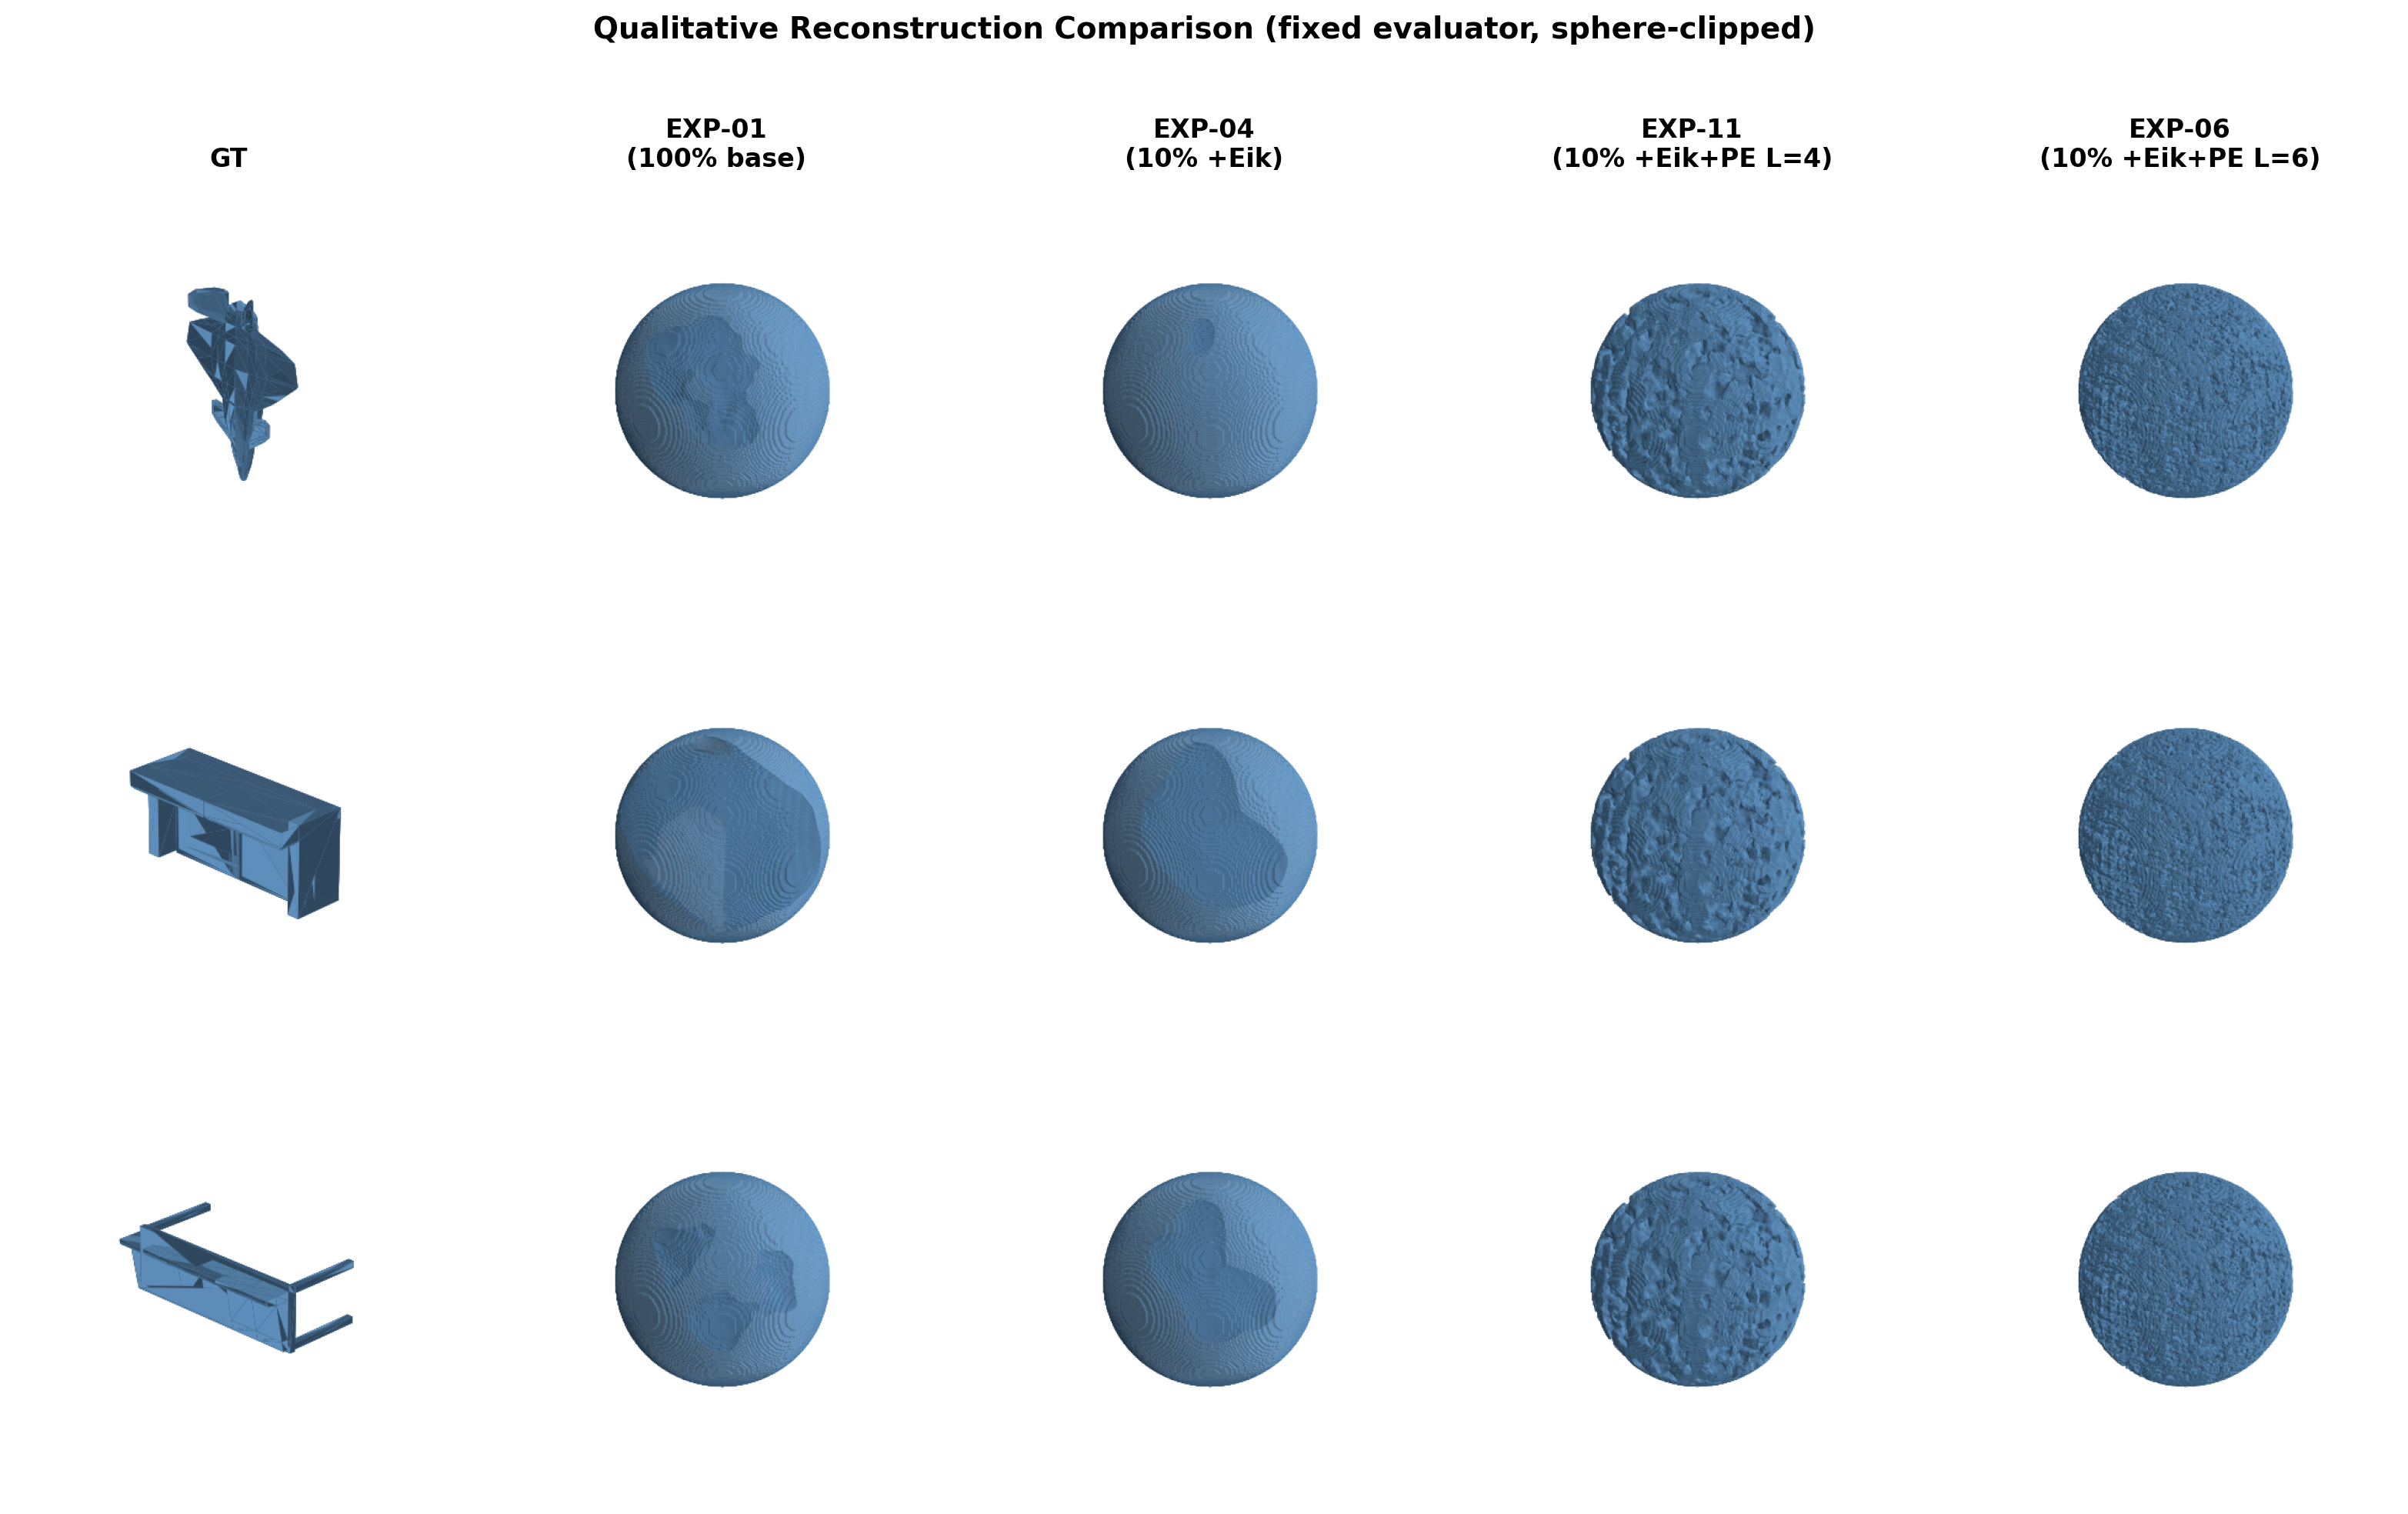
\includegraphics[width=\columnwidth]{figures/qualitative_meshes.png}
    \caption{Representative reconstructions from the corrected post-fix meshes.
    The 50\% + Eikonal column preserves recognizable structure more consistently
    than the 10\% condition, while the PE columns remain visibly poor.}
    \label{fig:qualitative}
\end{figure}

\begin{figure*}[t]
    \centering
    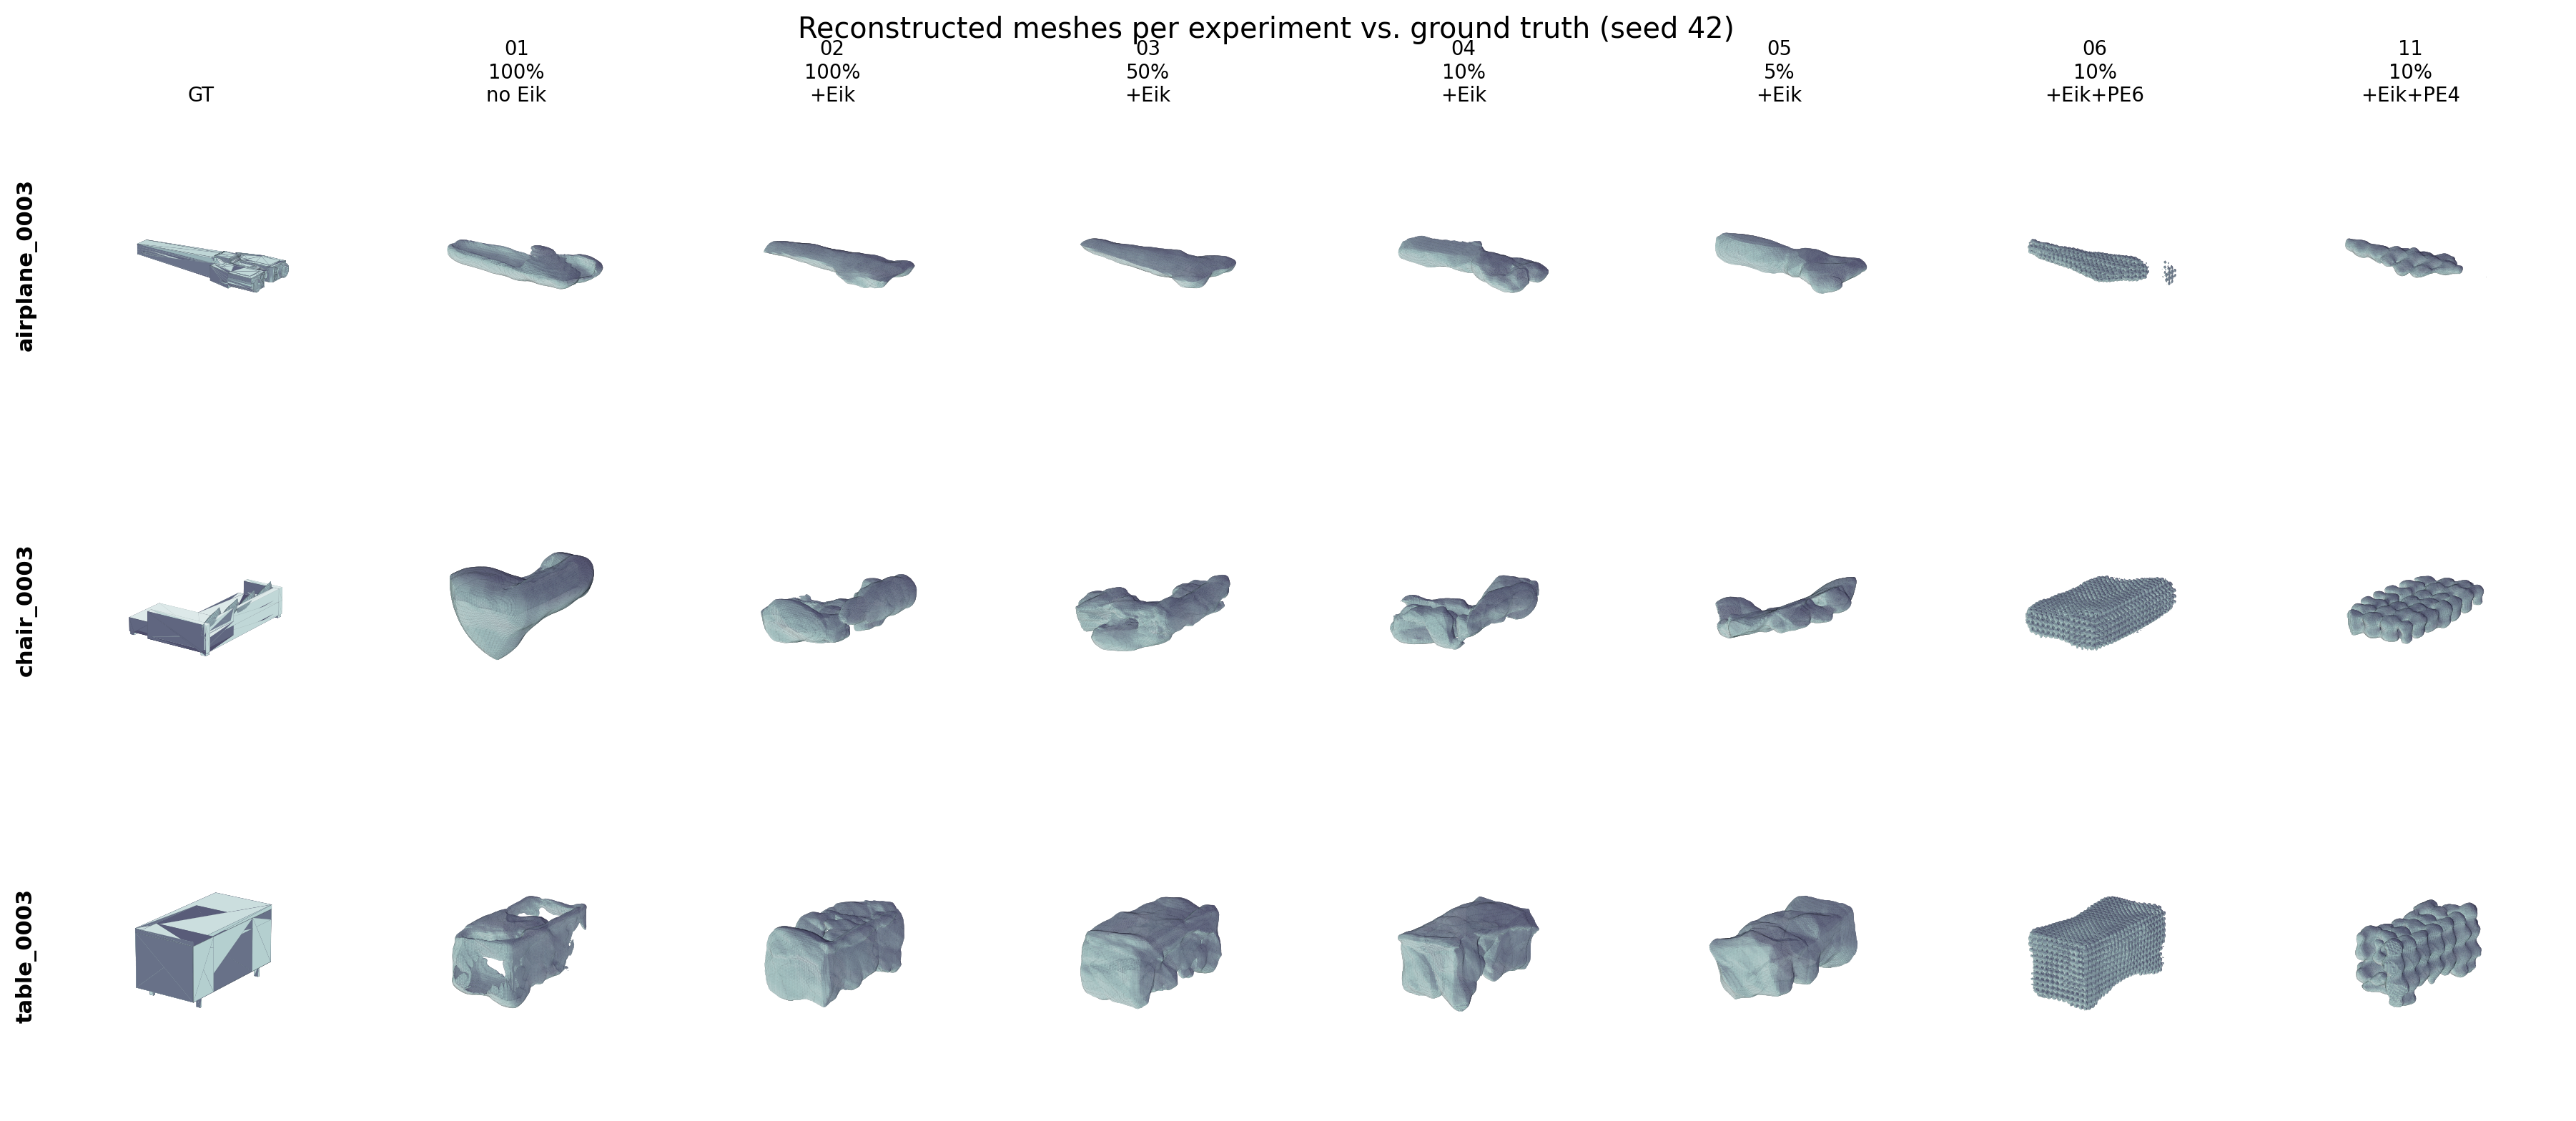
\includegraphics[width=\textwidth]{figures/mesh_comparison.png}
    \caption{Representative reconstructions by experiment. Qualitatively, the
    no-PE Eikonal runs improve over the baseline, but the 50\% condition is
    more structurally faithful than the 10\% condition. The PE columns are
    uniformly poor: thin structure disappears, surfaces become unstable, and
    reducing the PE frequency does not repair the failure mode.}
    \label{fig:mesh_comparison}
\end{figure*}

\subsection{Fourier PE Degrades Normal Consistency at 10\% Supervision}
\label{sec:pe_results}

Post-fix PE evidence is restricted to the 10\% supervision slice: EXP-06 at $L=6$ (3 seeds) and EXP-11 at $L=4$ (single seed). The originally-planned PE points at 5\% and 100\% supervision (EXP-07/EXP-09/EXP-10/EXP-12) and the second-order regularizer ablation (EXP-08) were not retrained on the corrected pipeline within the TC2 QoS budget; pre-fix exploratory results for those slots are kept in the experiment log for provenance only and are not used here.

Within the 10\% slice, the dominant effect of PE is on normal consistency rather than chamfer distance. EXP-06 reaches CD = 0.0308 $\pm$ 0.0012 across three seeds, almost identical to the no-PE EXP-04 value of 0.0315 $\pm$ 0.0015, while NC drops from 0.7288 $\pm$ 0.0032 (EXP-04) to 0.5171 $\pm$ 0.0066. EXP-11 with the lower PE frequency $L=4$ reaches CD = 0.0432 and NC = 0.6090, partially recovering NC at a modest CD cost. The PE-induced NC drop is reproducible across all three EXP-06 seeds (CV(NC) $\approx$ 0.013).

This is a narrower claim than the pre-fix draft suggested. We cannot state from corrected data that PE collapses CD across supervision ratios; we can state that, at 10\% supervision, PE primarily degrades the gradient field of the learned SDF (NC) rather than the surface localization itself (CD).

\subsection{PE Frequency Ablation at 10\% Supervision}

Within the post-fix 10\% slice, lowering the PE frequency from $L=6$ to $L=4$ partially recovers NC at the cost of higher CD. EXP-11 ($L=4$) achieves CD = 0.0432 and NC = 0.6090 against EXP-06's CD = 0.0308 $\pm$ 0.0012 and NC = 0.5171 $\pm$ 0.0066. So lowering $L$ moves the operating point toward the no-PE baseline on NC but away from it on CD, rather than producing a uniformly better PE configuration. The $L=4$ counterparts at 5\% and 100\% supervision were not retrained under the post-fix budget, so we cannot generalize this trend across supervision ratios.

\subsection{Per-Category Breakdown}
\label{sec:per_category}

Fig.~\ref{fig:per_category} breaks down the post-fix no-PE subset and the 10\% PE runs into per-shape CD and NC distributions by ShapeNet category. Three observations reinforce the aggregate numbers. (i)~Category difficulty is consistent: airplanes are the easiest and tables the hardest on CD across nearly every run, matching the intuitive geometric-complexity ordering. (ii)~Eikonal regularization compresses the category spread on both CD and NC (EXP-02 and EXP-03), i.e.\ its benefit is broadly distributed rather than concentrated in one category. (iii)~The NC drop under Fourier PE (EXP-06, EXP-11) is broadly distributed across categories rather than driven by one category, consistent with PE acting on the decoder's gradient field rather than on category-specific geometry.

\begin{figure*}[t]
    \centering
    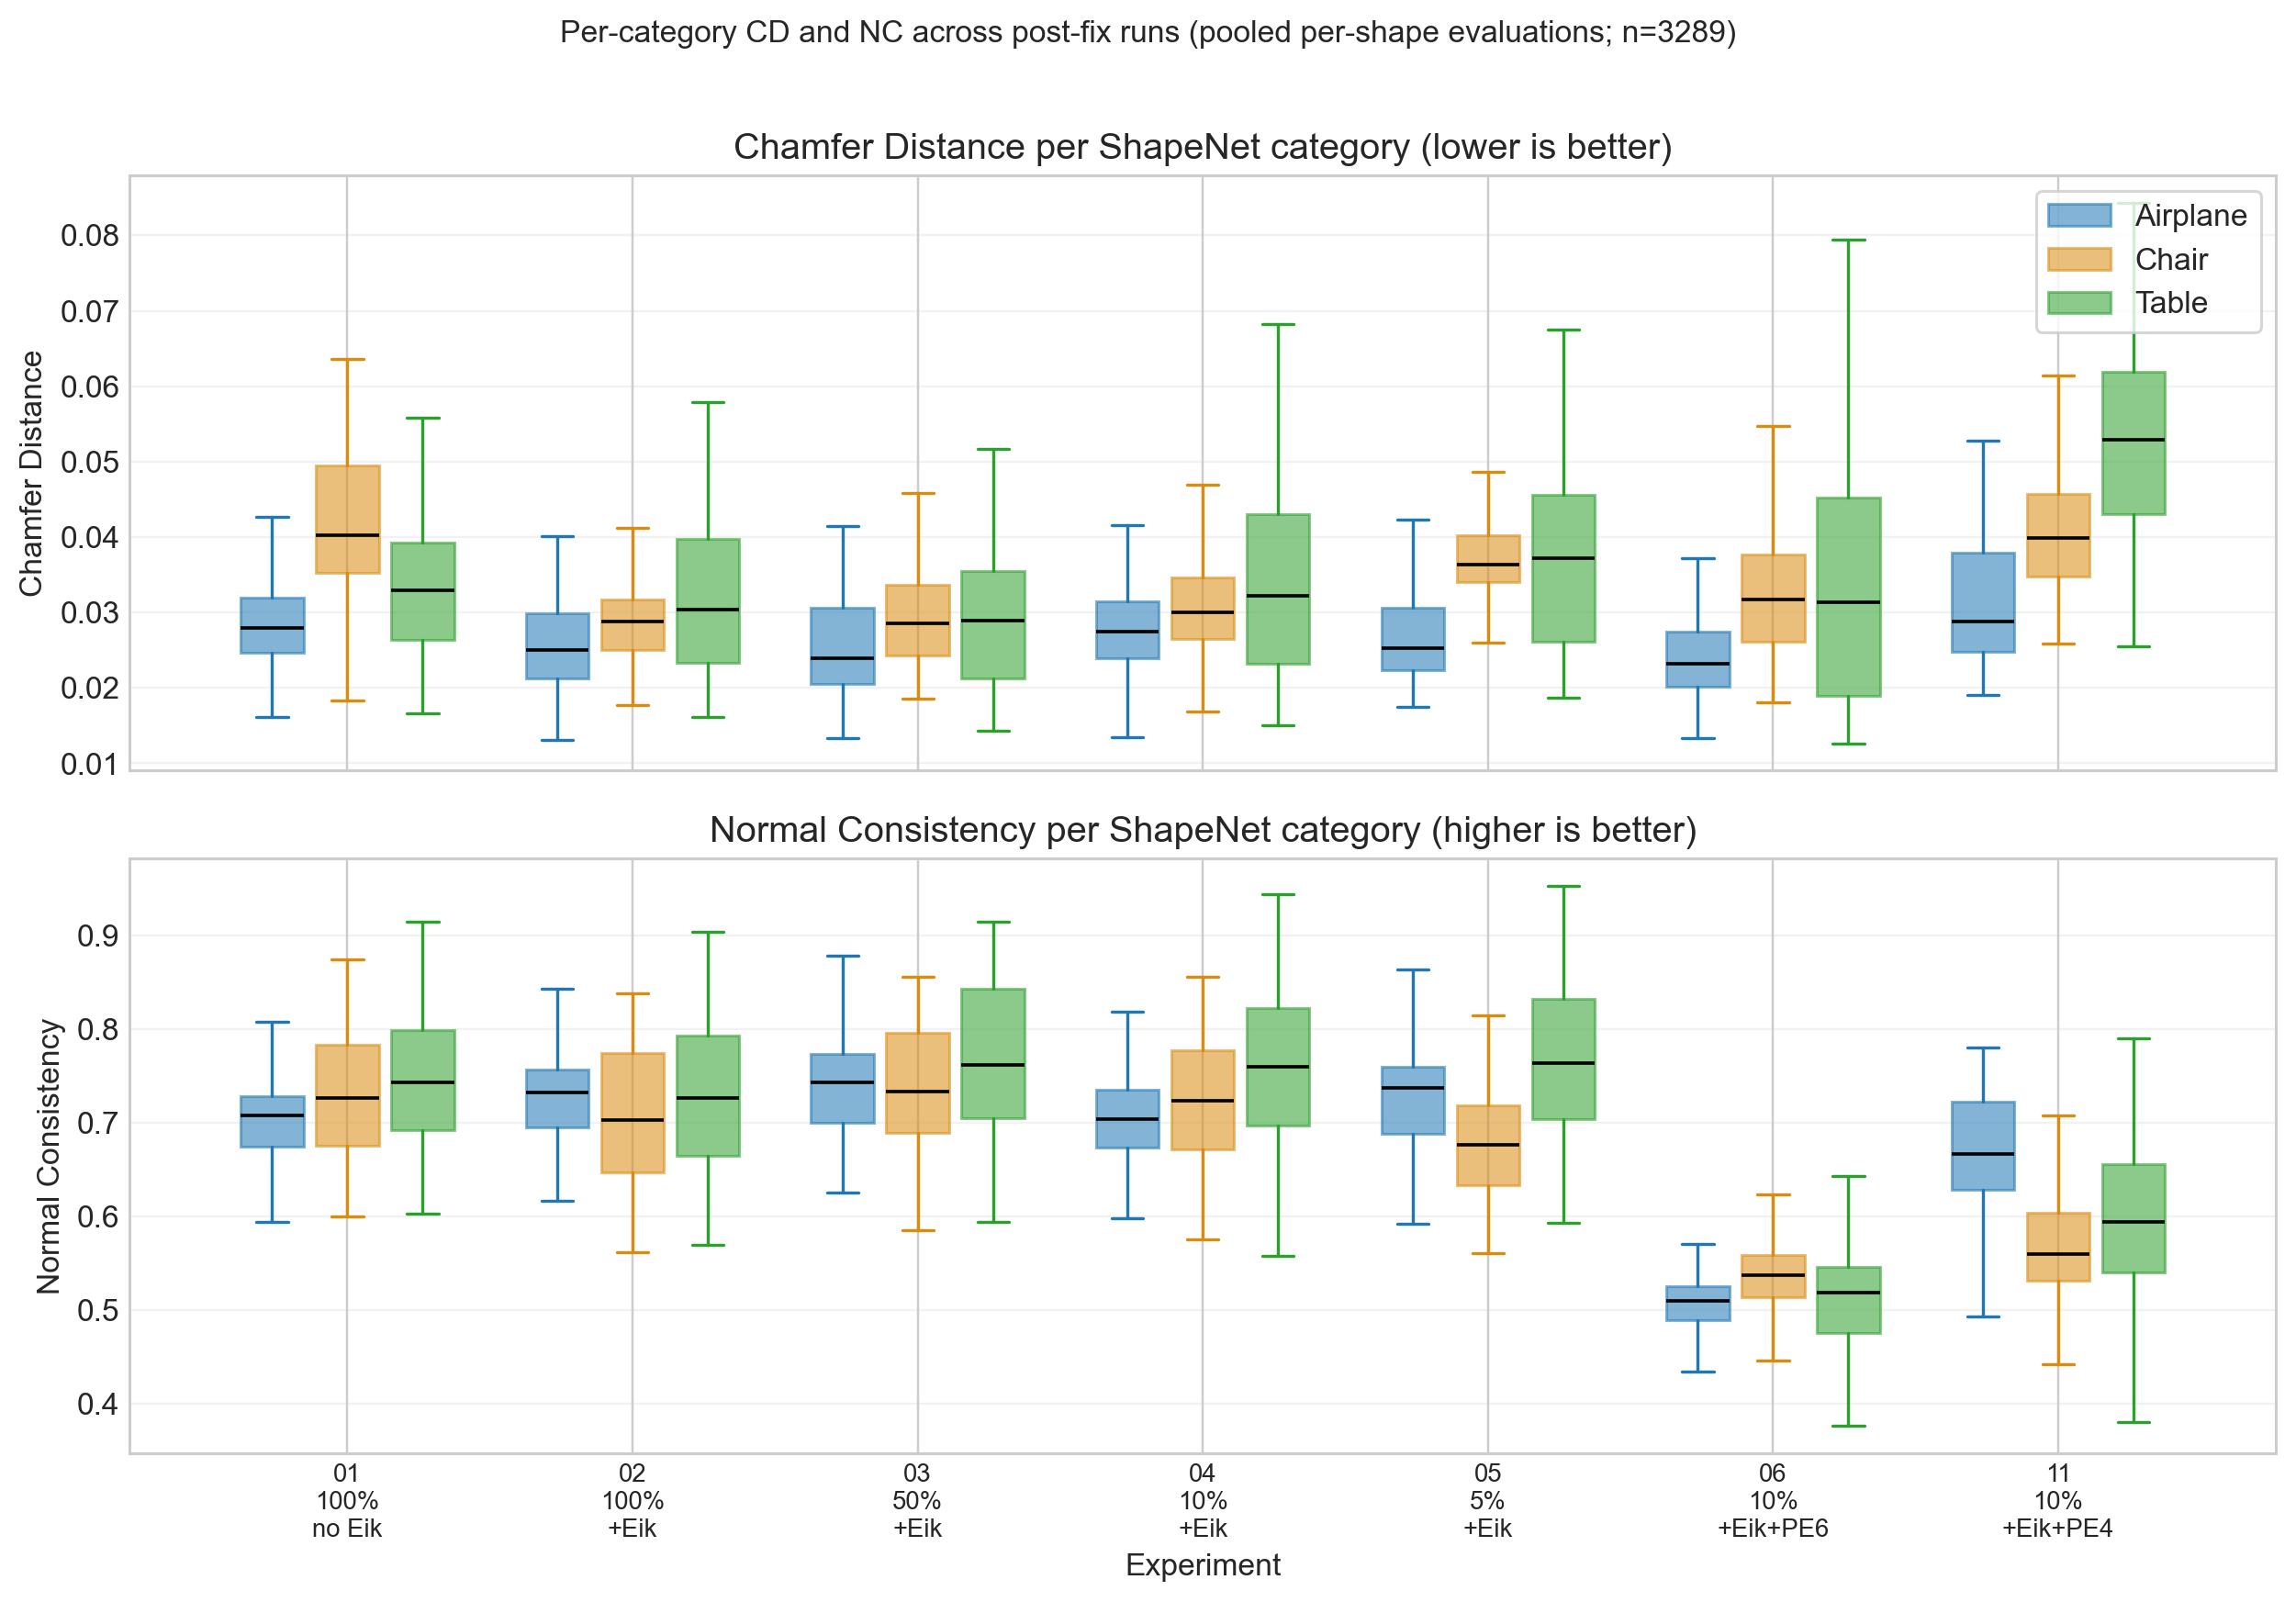
\includegraphics[width=\textwidth]{figures/per_category_cd_nc.png}
    \caption{Per-category subset visualization retained for qualitative
    support. The final report narrative uses Table~\ref{tab:results} as the
    authoritative source for the full experiment matrix.}
    \label{fig:per_category}
\end{figure*}

\subsection{Multi-Seed Validation}

We validated the two 10\%-supervision workhorse configurations with 3 seeds each (Table~\ref{tab:multiseed}). Both configurations are seed-stable (CV $<$ 0.05). EXP-06's NC drop relative to EXP-04 is reproducible across all three seeds, indicating that PE's effect on the gradient field is not driven by a single unlucky initialization.

\begin{table}[t]
\centering
\caption{Multi-seed validation (seeds 42, 123, 456). CV = coefficient of variation on CD.}
\label{tab:multiseed}
\renewcommand{\arraystretch}{1.1}
\footnotesize
\setlength{\tabcolsep}{3pt}
\begin{tabular}{@{}lcccc@{}}
\toprule
Experiment & CD mean & CD std & CV(CD) & NC mean \\
\midrule
04: 10\% + Eik & 0.0315 & 0.0015 & 0.047 & 0.7288 \\
06: 10\% + Eik + PE $L=6$ & 0.0308 & 0.0012 & 0.040 & 0.5171 \\
\bottomrule
\end{tabular}
\end{table}

\subsection{Excluded Early Pipeline}
\label{sec:preprocess_bug}

An early version of the pipeline sampled supervised SDF labels only inside a thin near-surface band, which made those results unsuitable for final interpretation. The final report therefore excludes all wrong-pipeline numbers. EXP-01 through EXP-06 and EXP-11 were retrained from scratch on the regenerated 80/20 near-surface plus far-field supervision and re-evaluated with the fixed evaluator. The originally-planned slots EXP-07 (5\% + PE $L=6$), EXP-08 (10\% + PE + $\mathcal{L}_{\text{2nd}}$), EXP-09 (100\% + PE $L=6$), EXP-10 (100\% + PE $L=4$), and EXP-12 (5\% + PE $L=4$) were not retrained under the post-fix QoS budget. Their pre-fix archived numbers are kept in the experiment log for provenance only and are not used in any table, figure, or conclusion in this paper.

%% ============================================================
\section{Discussion}
%% ============================================================

\subsection{Why Eikonal Enables Label Reduction}
\label{sec:why_eikonal}

The clearest claim the corrected data support is that Eikonal regularization
improves label efficiency relative to the non-Eikonal baseline. EXP-02 shows
that Eikonal already helps at full supervision, and EXP-03 shows that the model
can retain strong quantitative and qualitative structure even after halving the
labels. The 10\% and 5\% runs remain numerically competitive, but the figures
show that this should not be over-read as meaning all low-label reconstructions
are equally convincing.

We attribute this to the Eikonal term acting as a volumetric geometric prior. The supervised L1 SDF loss is by construction local: it only constrains $f_\theta$ at $N_s$ labeled points. When $N_s$ is small (25K supervised points per shape at 10\% supervision, 12.5K at 5\%), the decoder has enormous freedom in unsampled regions. The Eikonal term $(\|\nabla_x f\| - 1)^2$ removes that freedom in a specific way: it requires $f_\theta$ to be an honest distance function everywhere the gradient is evaluated, including on the 250K unsupervised points per shape. Practically, this closes two failure modes that hurt low-label DeepSDF: it prevents the decoder from collapsing away from the sparse labels (as the pre-fix preprocessing caused), and it penalizes high-curvature excursions between widely-spaced labeled points. The reason the 10\% + Eikonal run can match or beat 100\% + no-Eikonal is not that 10\% of the labels carry more signal than 100\%; it is that the Eikonal term extracts geometric regularization from the other 250K unsupervised points that the non-Eikonal baseline simply discards.

Two secondary observations support this interpretation. First, NC stays in the
approximately 0.72--0.75 band across the no-PE Eikonal runs, which is consistent with the
Eikonal term stabilizing the gradient field globally. Second, the ratio-dependent
warmup schedule appears necessary in practice, although we did not run a clean
ablation on warmup itself.

\subsection{Why Fourier PE Costs Normal Consistency}
\label{sec:why_pe}

The post-fix evidence at 10\% supervision is that Fourier PE primarily degrades the gradient field of the learned SDF. CD remains close to the no-PE baseline (EXP-06: 0.0308 vs EXP-04: 0.0315), but NC drops substantially (0.5171 vs 0.7288 at $L=6$). The NC drop is reproducible across three seeds (CV(NC) $\approx$ 0.013), so it is not seed-driven.

The most plausible explanation is that Fourier PE interacts badly with the training/evaluation geometry of this setup. The decoder is trained from near-surface structure inside the unit sphere, while normal computation requires a smooth gradient field over a dense extrapolation grid. With PE enabled, those coordinates appear to induce oscillatory behavior in the learned field that does not corrupt the zero level set itself (so CD survives) but does corrupt the gradient direction along it (so NC degrades).

Lowering the PE frequency from $L=6$ to $L=4$ partially mitigates the NC drop (EXP-11: NC = 0.6090) at the cost of a modestly higher CD (0.0432 vs 0.0308). We do not have post-fix evidence for whether this trade-off becomes more or less favorable at 5\% or 100\% supervision, and we therefore restrict the PE conclusion to the 10\% slice.

\subsection{Limitations}
\label{sec:limitations}

Several limitations of the post-fix study should be stated plainly.

\textbf{Training set evaluation only.} All CD/NC numbers are computed on the 299-shape training set rather than a held-out test split. The post-fix retrains used \texttt{train\_split}~=~1.0 because the study is scoped around the interaction between Eikonal regularization, Fourier PE, and supervision ratio on the training objective; generalization to unseen shapes is a separate question that we do not address.

\textbf{Uneven training budgets across phases.} EXP-01/02 used 3{,}000 epochs,
while the post-fix priority retrains (EXP-03/04/05/06/11) used 1{,}500 epochs
to fit the TC2 QoS budget. This does not invalidate the observed trends, but it
does make the matrix less uniform than an ideal final benchmark suite.

\textbf{Single dataset and small dataset scale.} We train on 299 shapes across three ShapeNet categories. Both the label-efficiency and PE-trade-off claims may behave differently at larger scale, with more categories, or on non-ShapeNet geometry.

\textbf{Incomplete post-fix PE matrix.} Only EXP-06 and EXP-11 (both at 10\% supervision) were retrained on the corrected pipeline within the available QoS budget. The PE points at 100\% and 5\% supervision (EXP-09/EXP-07/EXP-10/EXP-12) and the second-order regularizer ablation (EXP-08) are not in the post-fix evaluation, so the PE conclusion is restricted to the 10\% supervision slice.

\textbf{Metric coverage.} The original plan included volumetric IoU and an Eikonal-deviation metric ($|\|\nabla f\| - 1|$); neither was computed in the post-fix pipeline. Our conclusions are based on CD and NC only.

%% ============================================================
\section{Conclusion}
%% ============================================================

We set out to test whether Eikonal regularization can reduce the amount of
signed-distance supervision required by DeepSDF, and whether Fourier positional
encoding helps or hurts in that low-label regime. Using only the corrected
post-fix experiments, three conclusions are now clear. First, Eikonal
regularization is useful: it improves the full-label baseline and enables strong
performance at reduced supervision. Second, the most convincing label-efficiency
result is 50\% supervision with Eikonal, which combines the best no-PE metrics
with clearly recognizable reconstructions. Third, 10\% supervision with Eikonal
is promising numerically but should be described more cautiously because its
qualitative structure is less reliable than the 50\% case.

Fourier PE, by contrast, is not recommended at the supervision level we could test post-fix. At 10\% supervision, both PE configurations we retrained on the corrected pipeline (EXP-06 with $L=6$ and EXP-11 with $L=4$) degrade NC relative to the no-PE Eikonal baseline, with $L=4$ partially recovering NC at the cost of higher CD. The originally-planned PE points at 100\% and 5\% supervision (and the second-order regularizer ablation) were not retrained under the post-fix QoS budget, so we cannot generalize the PE finding across supervision ratios. The most natural next steps are therefore (i)~closing the post-fix PE matrix at 100\% and 5\% supervision and (ii)~exploring alternative high-frequency representations such as multi-resolution hash encodings~\cite{instantngp} or revised sampling strategies that reduce the observed mismatch between training support and reconstruction queries.

\begin{thebibliography}{00}
\bibitem{deepsdf} J.~J.~Park, P.~Florence, J.~Straub, R.~Newcombe, and S.~Lovegrove, ``DeepSDF: Learning continuous signed distance functions for shape representation,'' in \textit{Proc. IEEE/CVF CVPR}, 2019, pp.~165--174.

\bibitem{igr} A.~Gropp, L.~Yariv, N.~Haim, M.~Atzmon, and Y.~Lipman, ``Implicit geometric regularization for learning shapes,'' in \textit{Proc. ICML}, 2020, pp.~3789--3799.

\bibitem{nerf} B.~Mildenhall, P.~P.~Srinivasan, M.~Tancik, J.~T.~Barron, R.~Ramamoorthi, and R.~Ng, ``NeRF: Representing scenes as neural radiance fields for view synthesis,'' in \textit{Proc. ECCV}, 2020, pp.~405--421.

\bibitem{fourierfeatures} M.~Tancik \textit{et al.}, ``Fourier features let networks learn high frequency functions in low dimensional domains,'' in \textit{Proc. NeurIPS}, 2020, pp.~7537--7547.

\bibitem{siren} V.~Sitzmann, J.~N.~P.~Martel, A.~W.~Bergman, D.~B.~Lindell, and G.~Wetzstein, ``Implicit neural representations with periodic activation functions,'' in \textit{Proc. NeurIPS}, 2020, pp.~7462--7473.

\bibitem{shapenet} A.~X.~Chang \textit{et al.}, ``ShapeNet: An information-rich 3D model repository,'' \textit{arXiv preprint arXiv:1512.03012}, 2015.

\bibitem{marchingcubes} W.~E.~Lorensen and H.~E.~Cline, ``Marching cubes: A high resolution 3D surface construction algorithm,'' \textit{ACM SIGGRAPH Computer Graphics}, vol.~21, no.~4, pp.~163--169, 1987.

\bibitem{occnet} L.~Mescheder, M.~Oechsle, M.~Niemeyer, S.~Nowozin, and A.~Geiger, ``Occupancy Networks: Learning 3D reconstruction in function space,'' in \textit{Proc. IEEE/CVF CVPR}, 2019, pp.~4460--4470.

\bibitem{volsdf} L.~Yariv \textit{et al.}, ``Volume rendering of neural implicit surfaces,'' in \textit{Proc. NeurIPS}, 2021, pp.~4805--4815.

\bibitem{neus} P.~Wang \textit{et al.}, ``NeuS: Learning neural implicit surfaces by volume rendering for multi-view reconstruction,'' in \textit{Proc. NeurIPS}, 2021, pp.~27171--27183.

\bibitem{spectralbias} N.~Rahaman \textit{et al.}, ``On the spectral bias of neural networks,'' in \textit{Proc. ICML}, 2019, pp.~5301--5310.

\bibitem{instantngp} T.~M\"{u}ller, A.~Evans, C.~Schied, and A.~Keller, ``Instant neural graphics primitives with a multiresolution hash encoding,'' \textit{ACM Trans. Graphics}, vol.~41, no.~4, pp.~1--15, 2022.

\end{thebibliography}

\end{document}
